\documentclass[12pt]{article}
\usepackage{enumitem}
\usepackage{amsmath}
\usepackage{geometry}
\geometry{margin=1in}
\usepackage{listings}
\usepackage{graphicx}
\usepackage{xcolor} % for custom colors

\lstdefinestyle{mypython}{
    language=Python,
    basicstyle=\ttfamily\small,
    keywordstyle=\color{blue},
    stringstyle=\color{red},
    commentstyle=\color{green!50!black},
    showstringspaces=false,
    breaklines=true,
    backgroundcolor=\color{gray!10}, % light gray background
    frame=none                      % no border/frame
}

% Reduce spacing after \maketitle
\usepackage{etoolbox}
\makeatletter
\renewcommand{\maketitle}{
  \begin{center}
    {\Large \@title \par}
    \vskip 0.5em % space between title and date (reduce this as needed)
    {\@date}
  \end{center}
  \vskip 0em % space after date before text
}
\makeatother

\title{\Large Reproducing what J. Shao did}
\date{\today}

% Define shortcuts for bullet points


\begin{document}

\maketitle

\section{Plots}

The set of input parameters are: 
\begin{itemize}
    \item model parameters: $P_{crit}$, $m_s$, RMF model name (default RMF-QMC3), nuclear matter type (default pure neutron matter); The spot of model parameter $B_{SQM}^{1/4}$ is taken by the more physical $P_{crit}$
    \item dynamical parameters: $\Delta P$, $T$
    \item other default settings: masses $m_u = m_d = m_e = 0$, strong coupling $\alpha_s = 0.3$, in velocity formula: $\tau_Q = 1.3\times 10^{-9}\left(\frac{300\text{ MeV}}{\mu_Q}\right)^5$ s $ = 1.98\times 10^{12} \left(\frac{300\text{ MeV}}{\mu_Q}\right)^5$ MeV$^{-1}$, and $D_Q^{-1} = \frac{24~N_f~\alpha_s^2}{3 \pi} \Big(h \frac{T^{5/3}}{q_D^{2/3}} + \frac{\pi^3 T^2}{12 q_D} \Big)$. I work in natural units in MeV, then multiply speed of light to convert velocity in natural units to SI units. 
\end{itemize}
The parameters above should determine the value of phase boundary velocity. 

First, I'll plot contours of velocity varying dynamical parameters $\Delta P, T$ while fixing other parameters, the values of which are indicated as bullet points.

Then, I'll plot contours of velocity varying model parameters $m_s, P_{crit}$ while fixing $T, \Delta P$; the values are also listed in bullet points. 

For quark matter EoS, I added contributions from gluons, electrons, and the three quarks, enforcing charge neutrality. See Section~\ref{QM-EoS} for the code.


\newpage
\subsection{Contours varying dynamical parameters $\Delta P, T$}

\subsubsection{Contour plot-1}

\begin{itemize}
    \item $P_{crit} = 2\times 10^8$ MeV$^4$
    \item $m_s = 100$ MeV
    \item using RMF-QMC3 model for pure neutron matter
\end{itemize}

\begin{center}
    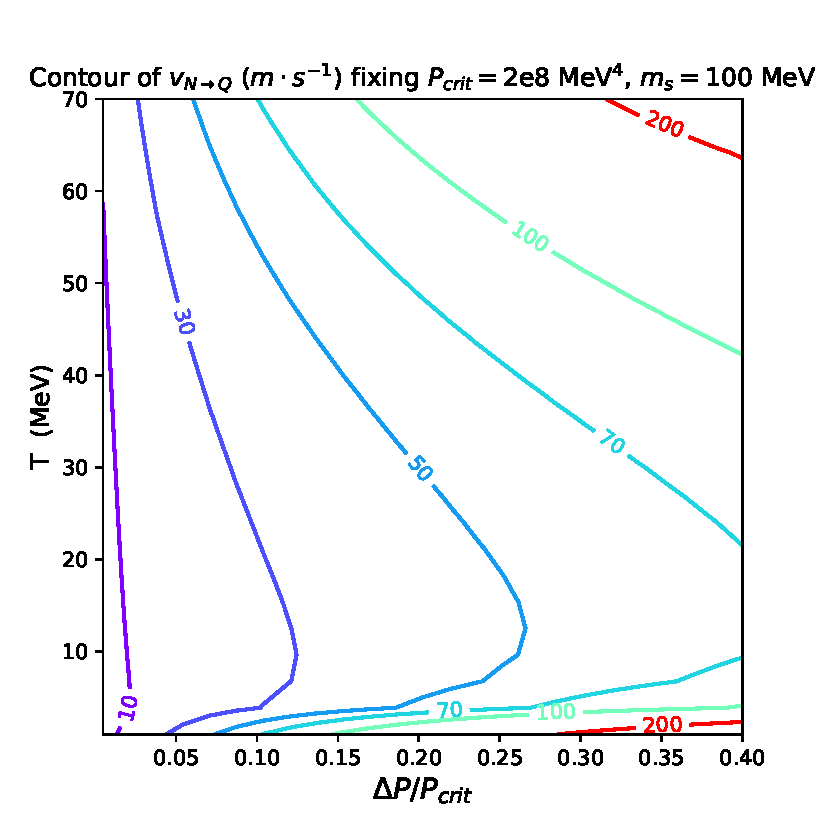
\includegraphics[width=1.0\textwidth]{DelP_T_Pcrit=2e8_ms=100_numerical.pdf} 
\end{center}

\newpage
\subsubsection{Contour plot-2}

\begin{itemize}
    \item $P_{crit} = 2\times 10^8$ MeV$^4$
    \item $m_s = 0$ MeV
    \item using RMF-QMC3 model for pure neutron matter
\end{itemize}

\begin{center}
    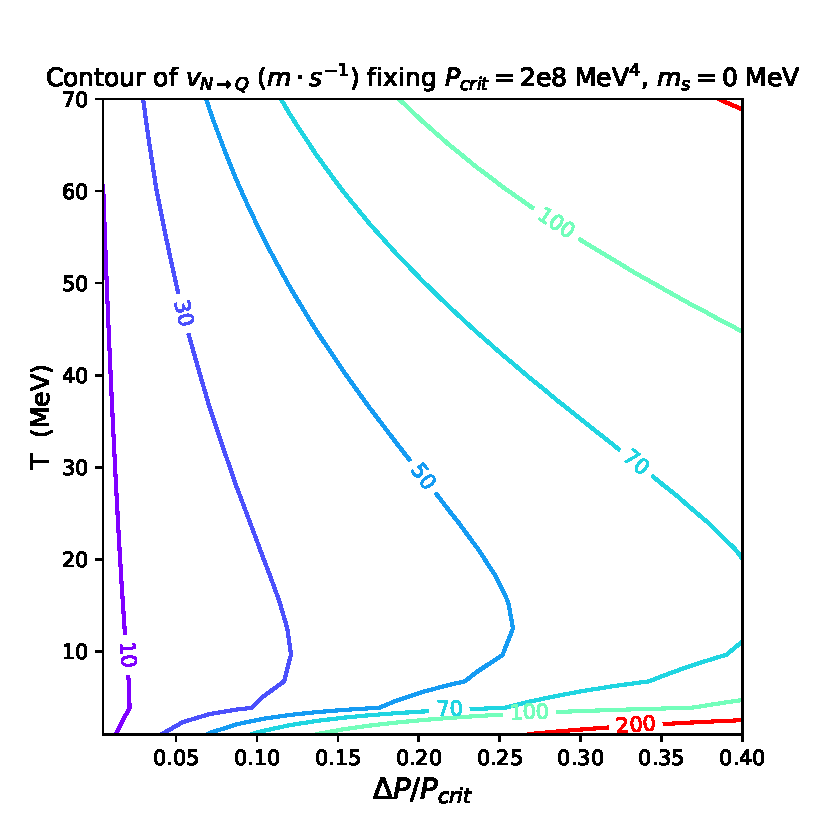
\includegraphics[width=1.0\textwidth]{DelP_T_Pcrit=2e8_ms=0_numerical.pdf} 
\end{center}

\newpage
\subsubsection{Contour plot-3}

\begin{itemize}
    \item $P_{crit} = 1\times 10^8$ MeV$^4$
    \item $m_s = 100$ MeV
    \item using RMF-QMC3 model for pure neutron matter
\end{itemize}

\begin{center}
    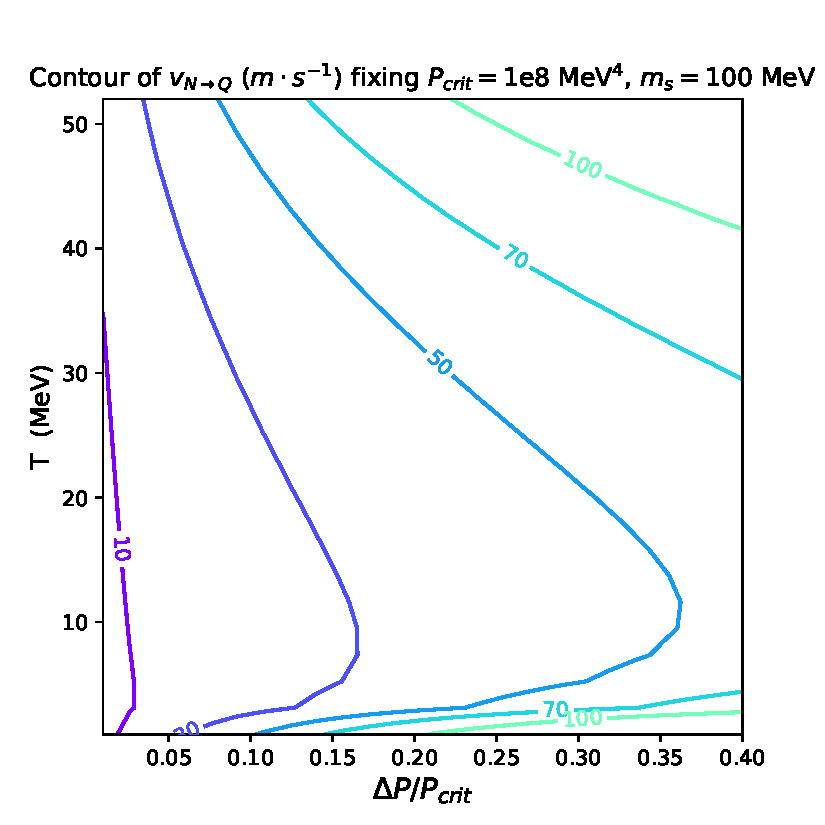
\includegraphics[width=1.0\textwidth]{DelP_T_Pcrit=1e8_ms=100_numerical.pdf} 
\end{center}

\newpage
\subsubsection{Contour plot-4}

\begin{itemize}
    \item $P_{crit} = 1\times 10^8$ MeV$^4$
    \item $m_s = 0$ MeV
    \item using RMF-QMC3 model for pure neutron matter
\end{itemize}

\begin{center}
    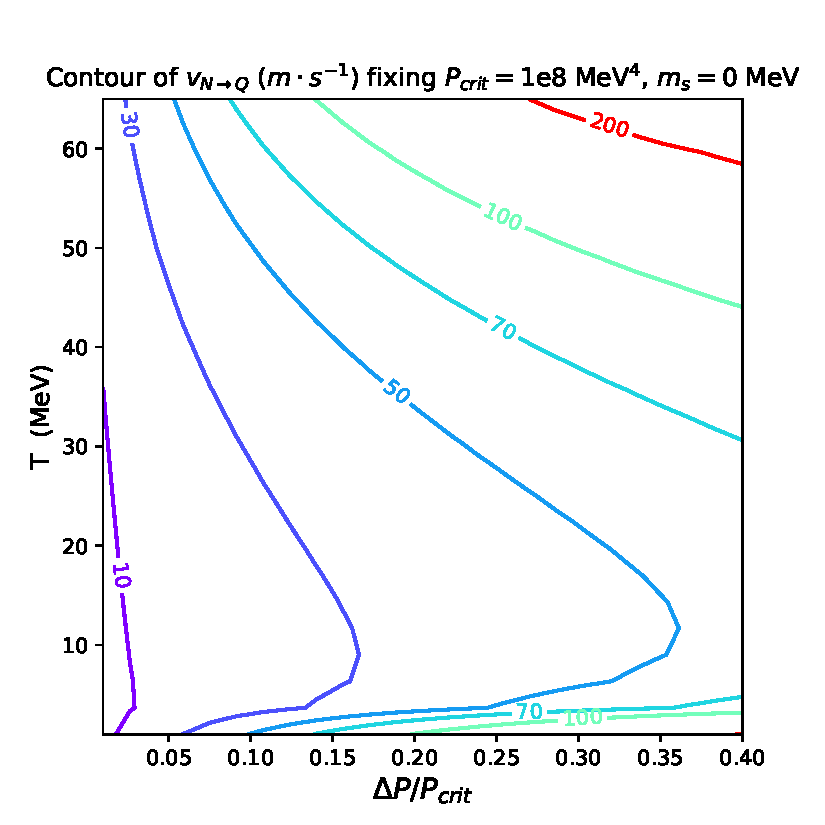
\includegraphics[width=1.0\textwidth]{DelP_T_Pcrit=1e8_ms=0_numerical.pdf} 
\end{center}

\newpage
\subsection{Contours varying model parameters $P_{crit}$, $m_s$}

\subsubsection{Contour plot-5}

\begin{itemize}
    \item $\Delta P = 1\times 10^7$ MeV$^4$
    \item $T = 10$ MeV
    \item using RMF-QMC3 model for pure neutron matter
\end{itemize}

\begin{center}
    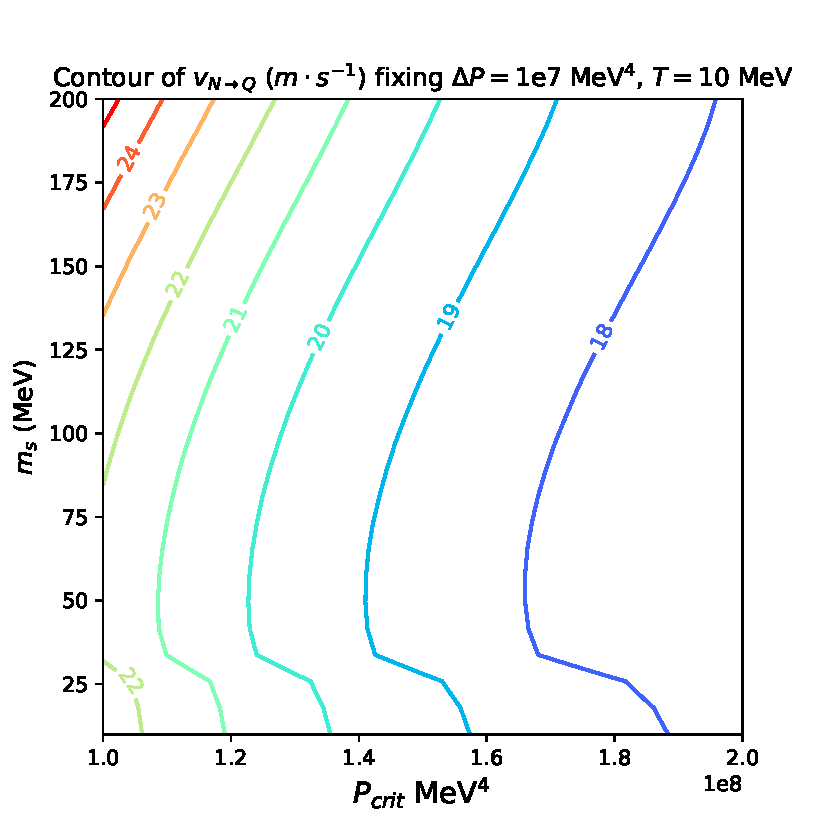
\includegraphics[width=1.0\textwidth]{MS_Pc_DelP=1e7_T=10_numerical.pdf} 
\end{center}


\newpage
\subsubsection{Contour plot-6}

\begin{itemize}
    \item $\Delta P = 1\times 10^7$ MeV$^4$
    \item $T = 20$ MeV
    \item using RMF-QMC3 model for pure neutron matter
\end{itemize}

\begin{center}
    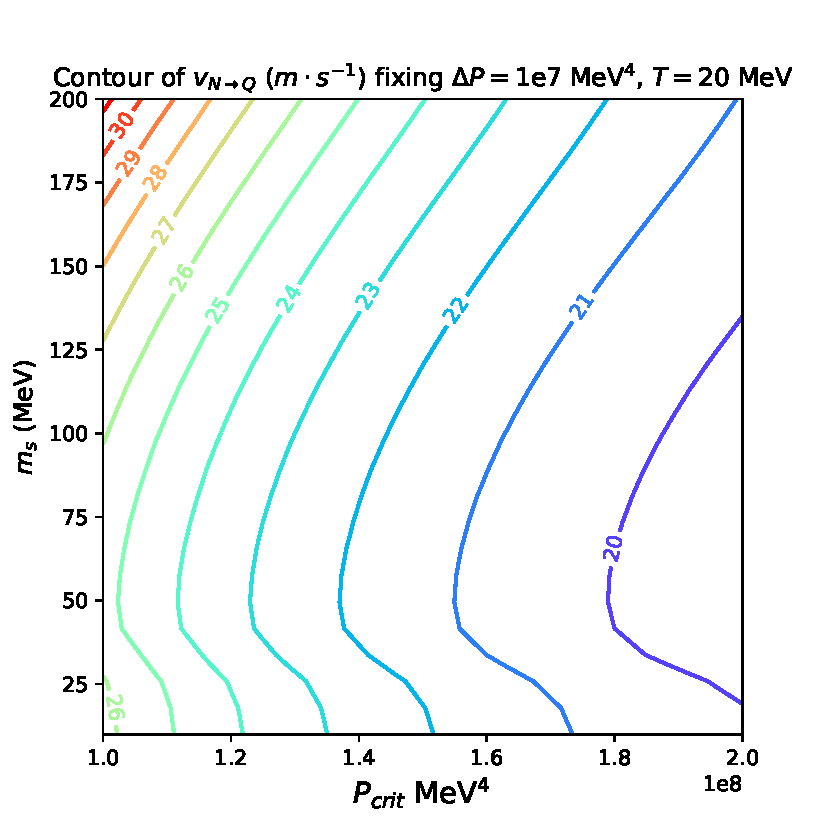
\includegraphics[width=1.0\textwidth]{MS_Pc_DelP=1e7_T=20_numerical.pdf} 
\end{center}


\newpage
\subsubsection{Contour plot-7}

\begin{itemize}
    \item $\Delta P = 5\times 10^7$ MeV$^4$
    \item $T = 10$ MeV
    \item using RMF-QMC3 model for pure neutron matter
\end{itemize}

\begin{center}
    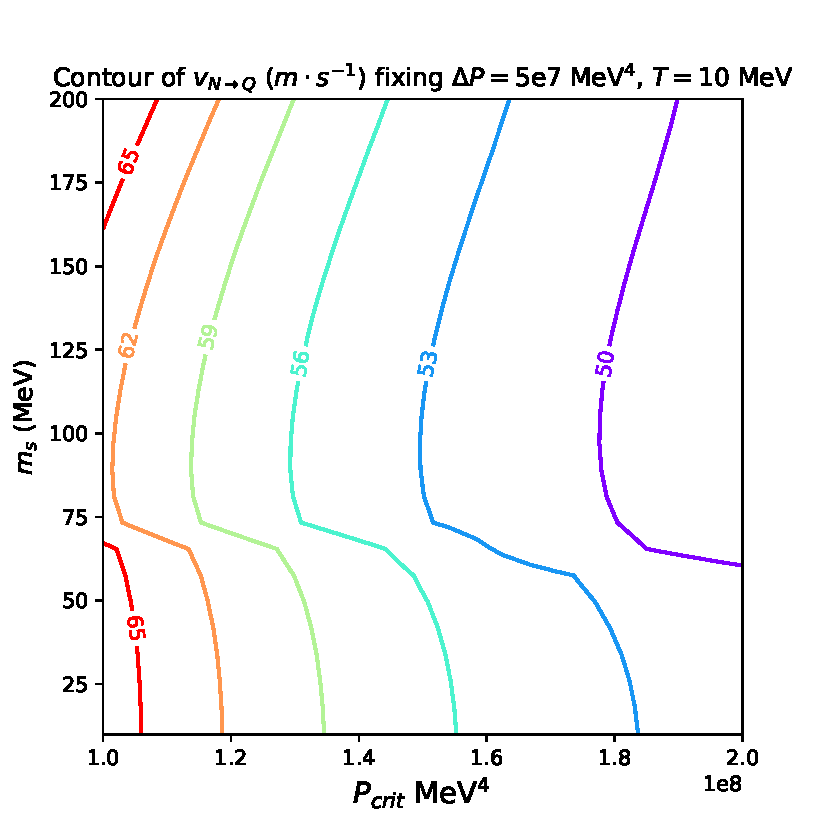
\includegraphics[width=1.0\textwidth]{MS_Pc_DelP=5e7_T=10_numerical.pdf} 
\end{center}


\newpage
\subsubsection{Contour plot-8}

\begin{itemize}
    \item $\Delta P = 5\times 10^7$ MeV$^4$
    \item $T = 20$ MeV
    \item using RMF-QMC3 model for pure neutron matter
\end{itemize}

\begin{center}
    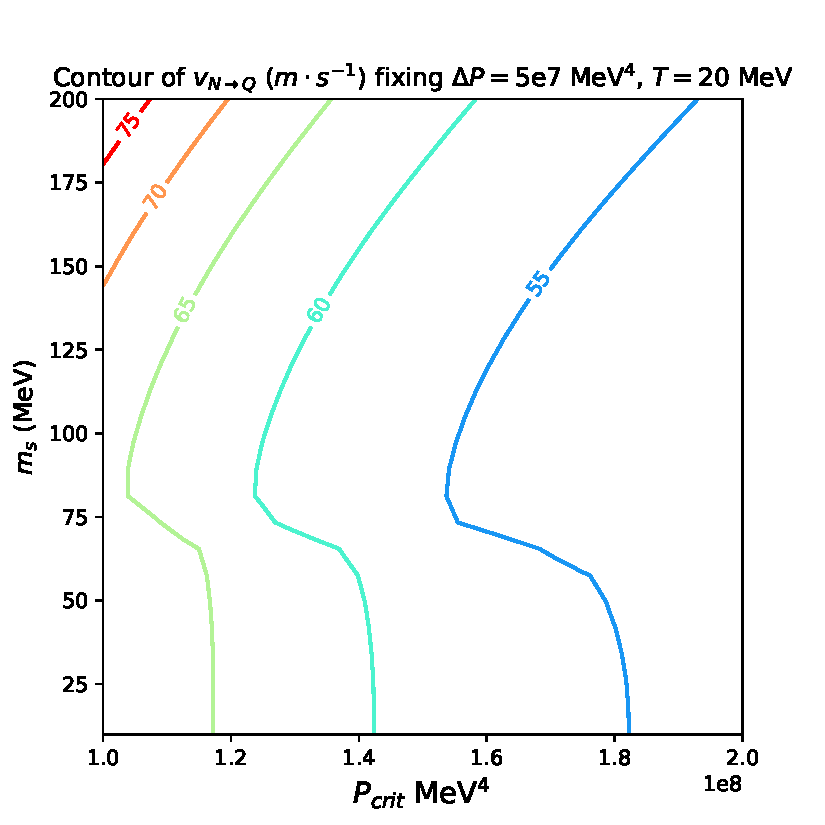
\includegraphics[width=1.0\textwidth]{MS_Pc_DelP=5e7_T=20_numerical.pdf} 
\end{center}


\newpage
\section{Relavant code for reference}

\subsection{Constants and parameters}

I defined the following in two separate .py files to be imported as packages. 

\begin{lstlisting}[style=mypython]
import math
import numpy as np

G  = 6.6730831e-8
c  = 2.99792458e10
MeV_fm3_to_pa = 1.6021766e35
c_km = 2.99792458e5 # km/s
mN = 1.67e-24 # g
mev_to_ergs = 1.602176565e-6
fm_to_cm = 1.0e-13
ergs_to_mev = 1.0/mev_to_ergs
cm_to_fm = 1.0/fm_to_cm
Msun = 1.988435e33
MeV_fm3_to_pa_cgs = 1.6021766e33
km_to_mSun = G/c**2

hbarc3 = 197.32700288295746**3

nucleon_mass = 938.04

pi = math.pi

# Fundamental conversions
MeV_fm = 197.326960
MeV_cm = MeV_fm * 1e-13
MeV_m = MeV_fm * 1e-15
MeV_km = MeV_cm * 1e-5
MeV_sec = 6.58212e-22

# Mass-energy conversion
MeV_per_gram = 5.60959e26
gram_per_MeV = 1 / MeV_per_gram
MeV_per_kg = 1000 * MeV_per_gram
kg_per_MeV = gram_per_MeV / 1000

# Dyne per MeV^2
dyne_per_MeV2 = gram_per_MeV * MeV_cm / MeV_sec**2
MeV2_per_dyne = 1 / dyne_per_MeV2

# Temperature-energy conversions
K_per_eV = 11605.
K_per_MeV = K_per_eV * 1e6
eV_per_K = 1 / K_per_eV
MeV_per_K = 1 / K_per_MeV

# Charge and energy
e_C = 1.60217646e-19  # Coulombs
J_per_eV = e_C
J_per_MeV = J_per_eV * 1e6
eV_per_J = 1 / J_per_eV
MeV_per_J = 1 / J_per_MeV

# Ergs
erg_per_MeV = 1e7 * J_per_MeV
MeV_per_erg = 1e-7 * MeV_per_J

# Speed of light and time
m_per_sec = 2.99792458e8
cm_per_sec = 100 * m_per_sec
sec_per_year = 31556925.9747

# Particle masses
Mneutron_MeV = 939.565378
Mneutron_gram = Mneutron_MeV * gram_per_MeV
Mproton_MeV = 938.272013
Mproton_gram = Mproton_MeV * gram_per_MeV
Melectron_MeV = 0.51100
Melectron_gram = Melectron_MeV * gram_per_MeV

# Weak interaction
G_Fermi = 1.16637e-11  # MeV^-2
Cabibbo_angle_rad = 13.02 * 2 * np.pi / 360

# Electromagnetism
epsilon_SI = 8.85418782e-12  # F/m
hbar_SI = 1.05457148e-34  # J.s
c_SI = 2.99792458e8  # m/s

# Magnetic conversions
MeV2_per_Tesla = np.sqrt(epsilon_SI * hbar_SI**3 * c_SI**5) / J_per_MeV**2
MeV2_per_Gauss = MeV2_per_Tesla / 1e4
Tesla_per_MeV2 = 1 / MeV2_per_Tesla
Gauss_per_MeV2 = 1 / MeV2_per_Gauss

# Nuclear densities
NuclearDensity_nucleons_per_fm3 = 0.16
NuclearDensity_nucleons_MeV3 = NuclearDensity_nucleons_per_fm3 * MeV_fm**3
NuclearDensity_quarks_MeV3 = 3 * NuclearDensity_nucleons_MeV3

# Energy density of nuclear matter
NuclearEnergyDensity_MeV4 = (Mneutron_MeV - 8) * NuclearDensity_nucleons_MeV3
NuclearEnergyDensity_g_per_cm3 = NuclearEnergyDensity_MeV4 / MeV_per_gram / MeV_cm**3

# Solar and astrophysical constants
MSolar_gram = 1.98847e33
MSolar_MeV = MSolar_gram * MeV_per_gram
BSolar = MSolar_MeV / Mneutron_MeV

# Newton's constant
NewtonG_SI = 6.67428e-11  # m^3 kg^-1 s^-2
NewtonG_MeV = NewtonG_SI / (hbar_SI * c_SI**5) * J_per_MeV**2  # MeV^-2
\end{lstlisting}

The second .py file in which different RMF model parameters are defined. The style is consistent with Alex's style. 

\begin{lstlisting}[style=mypython]
import numpy as np
import RMFsolver.constants as const # This imports the const file above. 

'''
Style for para:
para : list of lists/values
    Format:
    [
        [mn, mp],
        [ms, mw, mr],
        [I3n, I3p],
        [gsn, gsp],
        [gwn, gwp],
        [grn, grp],
        [b, c, Mn],
        [zet],
        [xi],
        [b1, b2, b3, a1, a2, a3, a4, a5, a6],
        nsat,
        bar,
        BagConst (optional)
    ]
'''


paraTMA=[[938.9,938.9],[519.151,781.95,768.1],[-.5,.5],[-10.055,-10.055],[12.842,12.842],[2*3.8,2*3.8],[0.328*const.MeV_fm/939/(10.055)**3,38.862/10.055**4,939],[151.590*6/12.842**4],[0],[0,0,0,0,0,0,0,0,0],0.147*const.MeV_fm**3,-1,0];
paraSFHo=[[939.565,938.272],[2.3689528914*const.MeV_fm,3.9655047020*const.MeV_fm,3.8666788766*const.MeV_fm],[-.5,.5],[2.3689528914*3.1791606374,2.3689528914*3.1791606374],[2.275188529*3.9655047020,2.275188529*3.9655047020],[2.4062374629*3.8666788766,2.4062374629*3.8666788766],[7.3536466626*10**(-3),-3.8202821956*10**(-3),939],[-1.6155896062*10**(-3)],[4.1286242877*10**(-3)],[5.5118461115,-1.8007283681*const.MeV_fm**(-2),4.2610479708*10**2*const.MeV_fm**(-4),-1.9308602647*10**(-1)*const.MeV_fm,5.6150318121*10**(-1),2.8617603774*10**(-1)*const.MeV_fm**(-1),2.7717729776*const.MeV_fm**(-2),1.2307286924*const.MeV_fm**(-3),6.1480060734*10**(-1)*const.MeV_fm**(-4)],0.1583*const.MeV_fm**3,-1,0];

const.MeV_fm_SFHoW=197.3269631;
paraSFHoWRONG=[[939.565346,938.272013],[2.3714*const.MeV_fm_SFHoW,762.5,770],[-.5,.5],[2.3714*3.1780,2.3714*3.1780],[762.5/const.MeV_fm_SFHoW*2.2726,762.5/const.MeV_fm_SFHoW*2.2726],[770/const.MeV_fm_SFHoW*2.4047,770/const.MeV_fm_SFHoW*2.4047],[7.4653*10**(-3),-4.0887*10**(-3),939],[-1.7013*10**(-3)],[3.4525*10**(-3)],[5.8729,-1.6442*const.MeV_fm_SFHoW**(-2),3.1464*10**2*const.MeV_fm_SFHoW**(-4),-2.3016*10**(-1)*const.MeV_fm_SFHoW,5.7972*10**(-1),3.4446*10**(-1)*const.MeV_fm_SFHoW**(-1),3.4593*const.MeV_fm_SFHoW**(-2),1.3473*const.MeV_fm_SFHoW**(-3),6.6061*10**(-1)*const.MeV_fm_SFHoW**(-4)],0.1583*const.MeV_fm_SFHoW**3,-1,0];

paraGM1=[[939,939],[550,783,770],[-.5,.5],[9.571775562457342,9.571775562457342],[10.611024696740092,10.611024696740092],[8.19657031394559,8.19657031394559],[0.002947,-0.00107,939],[0],[0],[0,0,0,0,0,0,0,0,0],0.153*const.MeV_fm**3,-1,0];

paraGM1SYM=[[939,939],[550,783,770],[-.5,.5],[np.sqrt(4*np.pi*6.003),np.sqrt(4*np.pi*6.003)],[np.sqrt(4*np.pi*5.948),np.sqrt(4*np.pi*5.948)],[0,0],[0.00795,0.0006952,939],[0],[0],[0,0,0,0,0,0,0,0,0],0.153*const.MeV_fm**3,-1,0];

paraIUF=[[939,939],[491.5,782.500,763.000],[-.5,.5],[np.sqrt(99.4266),np.sqrt(99.4266)],[np.sqrt(169.8349),np.sqrt(169.8349)],[np.sqrt(184.6877),np.sqrt(184.6877)],[3.3808/(2*939),0.000296/6,939],[0.03],[0],[0.046*169.8349,0,0,0,0,0,0,0,0],0.155*const.MeV_fm**3,-1,0];

paraTM1e=[[938,938],[511.19777,783,770],[-.5,.5],[-10.0289,-10.0289],[12.6139,12.6139],[13.9714,13.9714],[7.2325*const.MeV_fm/938/10.0289**3,0.6183/10.0289**4,938],[6*71.3075/12.6139**4],[0],[0.0429*12.6139**2,0,0,0,0,0,0,0,0],0.145*const.MeV_fm**3,-1,0]

# para=[[mn,mp],[m_sigma,m_omega,m_rho],[I3n,I3p],[gsn,gsp],[gwn,gwp],[grn,grp],[b,c,Mn_scale],[omega4_coupling],[rho4_coupling],[b1,b2,b3,a1,a2,a3,a4,a5,a6],nsat,bar,bag constant]; 
paraQMCRMF1=[[939,939],[491.5,782.5,763.],[-0.5,0.5],[7.54,7.54],[8.43,8.43],[10.88,10.88],[0.0073,0.0035,939],[0],[0],[7.89,0,0,0,0,0,0,0,0],1.2283363368456012e+6,-1,-612215];
paraQMCRMF2=[[939,939],[491.5,782.5,763.],[-0.5,0.5],[7.82,7.82],[8.99,8.99],[11.24,11.24],[0.0063,-0.0009,939],[0],[0],[8.02,0,0,0,0,0,0,0,0],1.2356201822425767e+6,-1,-463438];
paraQMCRMF3=[[939,939],[491.5,782.5,763.],[-0.5,0.5],[8.32,8.32],[9.76,9.76],[11.02,11.02],[0.0063,-0.006,939],[0],[0],[5.87,0,0,0,0,0,0,0,0],1.2053508748737855e+6,-1,-707480];
paraQMCRMF4=[[939,939],[491.5,782.5,763.],[-0.5,0.5],[8.21,8.21],[9.94,9.94],[12.18,12.18],[0.0041,-0.0021,939],[0],[0],[10.43,0,0,0,0,0,0,0,0],1.245066243773348e+6,-1,-206742];
paraQMCRMFx=[[1,paraQMCRMF1],[2,paraQMCRMF2],[3,paraQMCRMF3],[4,paraQMCRMF4]];

paraQMCRMF1_3D=[[939,939],[491.5,782.5,763.],[-0.5,0.5],[7.54,7.54],[8.43,8.43],[10.88,10.88],[0.0073,0.0035,939],[0],[0],[7.89,0,0,0,0,0,0,0,0],1.2283363368456012e+6,-1,-577307];
paraQMCRMF2_3D=[[939,939],[491.5,782.5,763.],[-0.5,0.5],[7.82,7.82],[8.99,8.99],[11.24,11.24],[0.0063,-0.0009,939],[0],[0],[8.02,0,0,0,0,0,0,0,0],1.2356201822425767e+6,-1,-460210];
paraQMCRMF3_3D=[[939,939],[491.5,782.5,763.],[-0.5,0.5],[8.32,8.32],[9.76,9.76],[11.02,11.02],[0.0063,-0.006,939],[0],[0],[5.87,0,0,0,0,0,0,0,0],1.2053508748737855e+6,-1,-723934];
paraQMCRMF4_3D=[[939,939],[491.5,782.5,763.],[-0.5,0.5],[8.21,8.21],[9.94,9.94],[12.18,12.18],[0.0041,-0.0021,939],[0],[0],[10.43,0,0,0,0,0,0,0,0],1.245066243773348e+6,-1,-150000];
paraQMCRMFx_3D=[[1,paraQMCRMF1_3D],[2,paraQMCRMF2_3D],[3,paraQMCRMF3_3D],[4,paraQMCRMF4_3D]];
\end{lstlisting}


\newpage
\subsection{Nuclear matter EoS calculation}

\subsubsection{Packages needed}
\begin{lstlisting}[style=mypython]
import numpy as np
from numpy.linalg import eigvals
from numdifftools import Derivative
from scipy.integrate import quad
from scipy.optimize import approx_fprime
from scipy.optimize import root
from scipy.interpolate import interp1d
from scipy.optimize import brentq
\end{lstlisting}

\subsubsection{Private functions}
First, private functions. I kept it as consistent as Alex's code as possible:
\begin{lstlisting}[style=mypython]
# para={{mn,mp},{m$sigma,m$omega,m$rho},{I3n,I3p},{gsn,gsp},{gwn,gwp},
# {grn,grp},{b,c,Mn$scale},{omega4$coupling},{rho4$coupling},
# {b1,b2,b3,a1,a2,a3,a4,a5,a6},nsat,bar};
def _set_couplings(para):
    """
    Set RMF model couplings and constants from a parameter list.

    Parameters:
    para : list of lists/values
        Format:
        [
            [mn, mp],
            [ms, mw, mr],
            [I3n, I3p],
            [gsn, gsp],
            [gwn, gwp],
            [grn, grp],
            [b, c, Mn],
            [zet],
            [xi],
            [b1, b2, b3, a1, a2, a3, a4, a5, a6],
            nsat,
            bar,
            BagConst (optional)
        ]
    """

    global ms, mw, mr, b, c, Mn, mB
    global gsn, gs, gw, gr, I3
    global zet, xi, bar
    global b1, b2, b3, a1, a2, a3, a4, a5, a6
    global me, upB, P_offset

    # Assignments
    ms = para[1][0]
    mw = para[1][1]
    mr = para[1][2]

    b = para[6][0]
    c = para[6][1]
    Mn = para[6][2]

    mB = para[0]
    gsn = para[3][0]
    gs = para[3]
    gw = para[4]
    gr = para[5]
    I3 = para[2]

    zet = para[7][0]
    xi = para[8][0]
    bar = -1

    b1, b2, b3, a1, a2, a3, a4, a5, a6 = para[9]

    me = 0.511  # Electron mass in MeV
    upB = 5000  # Upper integration bound

    P_offset = para[12] if len(para) > 12 and isinstance(para[12], (int, float)) else 0.0

def _fswr(sigma, w0):
    """
    Cross-coupling terms between rho/omega and rho/sigma, _set_couplings() should be called beforehand

    Parameters:
    sigma : scalar field (float)
    w0    : vector field (float)
    a1-a6 : coefficients for sigma terms
    b1-b3 : coefficients for w0 terms

    Returns:
    float : value of the cross-coupling potential
    """
    return (
        b1 * w0**2 + b2 * w0**4 + b3 * w0**6 +
        a1 * sigma + a2 * sigma**2 + a3 * sigma**3 +
        a4 * sigma**4 + a5 * sigma**5 + a6 * sigma**6
    )

def _U_sigma(s):
    """
    Sigma meson potential, _set_couplings() should be called beforehand

    Parameters:
    s    : sigma field value (float)
    ms   : sigma meson mass (float)
    gsn  : sigma-nucleon coupling constant (float)
    b, c : nonlinear self-interaction coefficients (float)
    Mn   : nucleon mass (float)

    Returns:
    float : value of the sigma potential
    """
    return (
        0.5 * ms**2 * s**2 +
        (b * Mn / 3) * (gsn * s)**3 +
        (c / 4) * (gsn * s)**4
    )

# meson lagrangian
def _Lmes(sigma, w0, r03, U_sigma_func=_U_sigma, fswr_func=_fswr):
    """
    Meson part of the Lagrangian density, _set_couplings() should be called beforehand.

    Parameters:
    sigma        : scalar mean field
    w0           : vector mean field
    r03          : isovector mean field
    mw, mr       : omega and rho meson masses
    zet, xi      : self-coupling coefficients
    gw, gr       : omega and rho coupling constants (e.g., gw[0], gr[0])
    U_sigma_func : function U_sigma(sigma)
    fswr_func    : function fswr(sigma, w0)

    Returns:
    float : meson Lagrangian value
    """
    return (
        -U_sigma_func(sigma) +
        0.5 * mw**2 * w0**2 +
        (zet / 24) * gw[1]**4 * w0**4 +
        0.5 * mr**2 * r03**2 +
        (xi / 24) * gr[1]**4 * r03**4 +
        gr[1]**2 * fswr_func(sigma, w0) * r03**2
    )

# baryon density for interacting baryons
def _nB(T, muB, BI, Sigma, w0, r03, upB=5000):
    """
    Calculate baryon density for species BI, _set_couplings() should be called beforehand.

    Parameters:
    T     : temperature (MeV)
    muB   : baryon chemical potential (MeV)
    BI    : baryon index
    Sigma : scalar mean field
    w0    : vector mean field
    r03   : isovector mean field
    upB   : upper momentum cutoff for integration
    mB    : list or array of baryon masses
    gs    : list or array of scalar couplings
    gw    : list or array of omega couplings
    gr    : list or array of rho couplings
    I3    : list or array of isospin values
    """

    # Effective mass and chemical potential
    m_eff = mB[BI] - gs[BI] * Sigma
    mu_eff = muB - gw[BI] * w0 - gr[BI] * I3[BI] * r03

    if T >= 0.1:
        def integrand(k):
            E_star = np.sqrt(k**2 + m_eff**2)
            term1 = k**2 / (1.0 + np.exp(np.clip((E_star - mu_eff) / T, -700, 700)))
            term2 = k**2 / (1.0 + np.exp(np.clip((E_star + mu_eff) / T, -700, 700)))
            return term1 - term2

        integral, _ = quad(integrand, 0, upB, limit=100, epsabs=1e-8, epsrel=1e-6)
        return integral / (np.pi**2)

    else:
        if mu_eff > m_eff:
            kF = np.sqrt(mu_eff**2 - m_eff**2)
            return kF**3 / (3 * np.pi**2)
        else:
            return 0.0

# scalar density 
def _ns(T, muB, BI, sigma, w0, r03, upB=5000):
    """
    Calculate baryon scalar density (source term for sigma meson).

    Parameters:
    T     : temperature (MeV)
    muB   : baryon chemical potential (MeV)
    BI    : baryon index (int)
    sigma : scalar field
    w0    : vector field
    r03   : isovector field
    mB, gs, gw, gr, I3 : model parameter arrays
    upB   : upper bound for momentum integration (default 5000 MeV)

    Returns:
    float : baryon scalar density
    """

    m_eff = mB[BI] - gs[BI] * sigma
    mu_eff = muB - gw[BI] * w0 - gr[BI] * I3[BI] * r03

    if T >= 0.1:
        def integrand(k):
            Ek = np.sqrt(k**2 + m_eff**2)
            f  = 1 / (1 + np.exp(np.clip((Ek - mu_eff) / T, -700, 700)))
            fbar = 1 / (1 + np.exp(np.clip((Ek + mu_eff) / T, -700, 700)))
            return (m_eff / Ek) * k**2 * (f + fbar)

        integral, _ = quad(integrand, 0, upB, epsabs=1e-10, epsrel=1e-8, limit=200)
        return integral / np.pi**2

    else:
        if mu_eff <= m_eff:
            return 0.0
        kF = np.sqrt(mu_eff**2 - m_eff**2)
        term1 = m_eff * kF * mu_eff
        term2 = m_eff**3 * np.log((mu_eff + kF) / m_eff)
        return (term1 - term2) / (2 * np.pi**2)

# Fermi momentum for baryons in RMF, needs _set_couplings
def _kf_bar(sigma, w0, r03, muB, BI):
    """
    Compute Fermi momentum for baryon species BI in RMF.

    Parameters:
    sigma : scalar field
    w0    : vector field
    r03   : isovector field
    muB   : baryon chemical potential
    BI    : baryon index
    mB, gs, gw, gr, I3 : global model arrays (must be set via _set_couplings)

    Returns:
    float : Fermi momentum (MeV), or 0 if below threshold
    """

    m_eff = mB[BI] - gs[BI] * sigma
    mu_eff = muB - gw[BI] * w0 - gr[BI] * I3[BI] * r03

    if mu_eff > m_eff and m_eff > 0:
        return np.sqrt(mu_eff**2 - m_eff**2)
    else:
        return 0.0

# E_F^* for baryons = Sqrt[kf^2+m*^2] (no vector mean fields), 
# needs _set_couplings
def _Ef_bar(sigma, w0, r03, muB, BI):
    """
    Compute effective Fermi energy for baryon BI (scalar part only).

    Parameters:
    sigma : scalar field
    w0    : vector field
    r03   : isovector field
    muB   : baryon chemical potential
    BI    : baryon index
    mB, gs, gw, gr, I3 : global model arrays

    Returns:
    float : Effective Fermi energy (MeV)
    """

    kf = _kf_bar(sigma, w0, r03, muB, BI)
    m_eff = mB[BI] - gs[BI] * sigma
    return np.sqrt(kf**2 + m_eff**2)

# fermi dirac distribution
def _fd(E, mu, T):
    """
    Smooth Fermi-Dirac distribution, numerically stable even near T = 0.
    """
    if T <= 1e-6:
        return np.clip(float(E < mu), 1e-15, 1.0)
    z = np.clip((E - mu) / T, -700, 700)
    return np.clip(1.0 / (1.0 + np.exp(z)), 1e-15, 1.0)

# Fermi Dirac distribution for Baryons, 
def _fd_bar(k, sigma, w0, r03, muB, BI, T):
    """
    Fermi-Dirac distribution for baryons in RMF.

    Parameters:
    k     : momentum
    sigma : scalar field
    w0    : vector field
    r03   : isovector field
    muB   : baryon chemical potential
    BI    : baryon index
    T     : temperature
    mB, gs, gw, gr, I3 : model parameter arrays

    Returns:
    float : Fermi-Dirac occupation number
    """
    m_eff = mB[BI] - gs[BI] * sigma
    mu_eff = muB - gw[BI] * w0 - gr[BI] * I3[BI] * r03
    E = np.sqrt(k**2 + m_eff**2)

    if T < 1e-3:
        return float(E < mu_eff)

    z = np.clip((E - mu_eff) / T, -700, 700)
    return 1.0 / (1.0 + np.exp(z))
\end{lstlisting}


\subsubsection{PNM RMF solver and EoS}

This is the RMF solver for PNM given $\mu_B$ as input. Since Alex's code takes $n_B$ as input, I wrote another one taking $\mu_B$ as input. 
\begin{lstlisting}[style=mypython]
# module to solve PNM RMFs given baryon chemical potential
def RMFsolvePNM_mu(mub, Trmf, para, sigma_init, w0_init, r03_init, verb=False):
    """
    Solve RMF for pure neutron matter (PNM) given baryon chemical potential.

    Parameters
    ----------
    mub  : float
        Baryon chemical potential.
    Trmf : float
        Temperature in MeV.
    para : list
        RMF model parameter set.
    sigma_init, w0_init, r03_init : float
        Initial guesses for sigma, omega_0, rho_03.
    verb : bool
        Verbosity flag.

    Returns
    -------
    list
        Solution structure: [[sigma, w0, r03, mu_n, 0, 0], [Eq1, Eq2, Eq3, 0, 0], T, n_B, para]
    """
    _set_couplings(para)

    if verb and Trmf <= 0.1:
        print("Temperature is either 0 or T < 1 MeV, T too small for finite T numerical integration, T=0 RMF solver is used")

    def Eq1(sigma, w0, r03):
        dLmes_dsigma = Derivative(lambda s: _Lmes(s, w0, r03))(sigma)
        return float(-gs[0] * _ns(Trmf, mub, 0, sigma, w0, r03) - dLmes_dsigma)

    def Eq2(sigma, w0, r03):
        dLmes_dw0 = Derivative(lambda w: _Lmes(sigma, w, r03))(w0)
        return float(-gw[0] * _nB(Trmf, mub, 0, sigma, w0, r03) + dLmes_dw0)

    def Eq3(sigma, w0, r03):
        dLmes_dr03 = Derivative(lambda r: _Lmes(sigma, w0, r))(r03)
        return float(-gr[0] * I3[0] * _nB(Trmf, mub, 0, sigma, w0, r03) + dLmes_dr03)

    def equations(x):
        sigma, w0, r03 = x
        return np.array([
            Eq1(sigma, w0, r03),
            Eq2(sigma, w0, r03),
            Eq3(sigma, w0, r03)
        ], dtype=float)

    x0 = [float(sigma_init), float(w0_init), float(r03_init)]
    sol = root(equations, x0, method='hybr', options={'maxfev': 60000})

    if not sol.success:
        #if verb:
        print("Root finding failed:", sol.message)
        raise RuntimeError("RMFsolvePNM_mu failed to converge")

    sigma, w0, r03 = sol.x
    chk = equations(sol.x)
    nb = _nB(Trmf, mub, 0, sigma, w0, r03)

    output = [[sigma, w0, r03, mub, 0.0, 0.0], list(chk) + [0, 0], Trmf, nb, para]

    if verb:
        if max(abs(c) for c in chk) > 1e-6:
            print("Accuracy not achieved, check functions > 10^(-6)")
        else:
            return output
    return output
\end{lstlisting}


The following calculates the PNM pressure. It can take $\mu_B$ as well as $n_B$ as input. When taking $n_B$ as input, it uses the RMF solver for PNM very same to Alex's one.
\begin{lstlisting}[style=mypython]
# module to solve RMF AND compute pressure PNM
def RMFpressurePNM(input_num, input_type, Trmf, para, sigma_init, w0_init, r03_init, mub_init, verb=True):
    """
    Compute pressure in pure neutron matter (PNM) using RMF solution.

    Parameters
    ----------
    input_num  : float
        Either baryon number density or baryon chemical potential
    inpyt_type : string
        "muB"  : for baryon chemical potential input
        "nB"   : for baryon number density input
    Trmf : float
        Temperature in MeV.
    para : list
        RMF model parameter set.
    sigma_init, w0_init, r03_init, mub_init : float
        Initial guesses for mean fields and chemical potential.
    verb : bool
        Verbosity flag.

    Returns
    -------
    float
        Total pressure (meson + neutron).
    """
    _set_couplings(para)

    if input_type == "nB":
        vevs = RMFsolvePNM(input_num, Trmf, para, sigma_init, w0_init, r03_init, mub_init, verb)

    elif input_type == "muB":
        vevs = RMFsolvePNM_mu(input_num, Trmf, para, sigma_init, w0_init, r03_init, verb)

    else:
        print("Unknown input type")
        return None

    chk = vevs[1]
    sigma = vevs[0][0]
    w0 = vevs[0][1]
    r03 = vevs[0][2]
    mub = vevs[0][3]
    muv = [mub, 0.0]  # only neutron contributes

    meson_pressure = _Lmes(sigma, w0, r03)
    nuc_pressure = nucleon_pressure(Trmf, muv[0], sigma, w0, r03, BI=0)

    if verb:
        if max(abs(c) for c in chk) > 1e-6:
            print("Accuracy not achieved, check functions > 10^(-6)")
        else:
            return meson_pressure + nuc_pressure

    return meson_pressure + nuc_pressure
\end{lstlisting}



\section{QM EoS and Pressure}

\subsection{Private functions}

\begin{lstlisting}[style=mypython]
# pressure for a single free fermion
def P_f(mu, m, Tem, upB=5000):
    '''
    Computes pressure for a single fermion species

    Parameters:
    - mu   : fermion chemical potential
    - m    : fermion mass
    - Tem  : temperature
    - upB  : upper limit for infinite integral, default=5000

    Returns:
    - pressure of this fermion species
    '''

    if Tem > 0.2:
        def integrand(k):
            Ek = np.sqrt(k**2 + m**2)
            arg = Tem * np.log(1 + np.exp(-np.clip((Ek - mu)/Tem, -700, 700)))
            arg_bar = Tem * np.log(1 + np.exp(-np.clip((Ek + mu)/Tem, -700, 700)))
            return (arg + arg_bar) * k**2

        integral, _ = quad(integrand, 0, upB, epsabs=1e-10, epsrel=1e-8)

        return integral / (np.pi**2)

    else:
        if m < 1e-3:
            return mu**4 / (12 * np.pi**2)
        else:
            k_F = np.sqrt(mu**2 - m**2)
            return ((2*k_F**3 - 3*m**2*k_F)*mu + 3*m**4*np.log((k_F+mu)/m)) / (24*np.pi**2)

# number density for a single free fermion
def n_B(mu, m, Tem, upB=5000):
    '''
    Returns number density for a single fermion species.
    Uses thermodynamic relation: dP/dmu = n
    '''

    if Tem > 0.2:
        def integrand(k):
            Ek = np.sqrt(k**2 + m**2)
            f = 1 / (1 + np.exp(np.clip((Ek - mu)/Tem, -700, 700)))
            f_bar = 1 / (1 + np.exp(np.clip((Ek + mu)/Tem, -700, 700)))
            return (f - f_bar) * k**2

        integral, _ = quad(integrand, 0, upB, epsabs=1e-10, epsrel=1e-8)

        return integral / (np.pi**2)

    else:
        k_F = np.sqrt(mu**2 - m**2)
        return k_F**3 / (3 * np.pi**2)
\end{lstlisting}

\subsection{QM pressure function}\label{QM-EoS}

\begin{lstlisting}[style=mypython]
# pressure for SQM under bag model
def PQM(muB, muK, B_one_forth, T, ms, upB=5000):
    '''
    Calculates the pressure of strange quark matter (SQM) under bag model

    Parameters:
    - muB         : baryon chemical potential, one third of average quark chemical potential
    - muK         : kaon-ness chemical potential, equals mu_d - mu_s
    - B_one_forth : bag constant for SQM bag model, input is B^(1/4)
    - T           : temperature
    - ms          : strange quark mass
    - upB         : integral upper bound

    Returns:
    - pressure for SQM matter
    '''

    B = B_one_forth**4
    mu_u = muB/3
    mu_d = muB/3 + muK/2
    mu_s = muB/3 - muK/2

    if ms > 1:
        n_u = n_B(mu_u, 0, T,)
        n_d = n_B(mu_d, 0, T,)
        n_s = n_B(mu_s, ms, T,)

        n_e = (2*n_u - n_d - n_s)/3
        solve_for_mu_e = lambda x: n_B(x, 0, T,) - n_e
        mu_e = fsolve(solve_for_mu_e, 100)[0]

    else:
        mu_e = 0

    return float( 16*np.pi**2*T**4 / 90 + P_f(mu_e, m=0, Tem=T) + 3*P_f(mu_u, m=0, Tem=T) + 3*P_f(mu_d, m=0, Tem=T) + 3*P_f(mu_s, ms, Tem=T) - B )
\end{lstlisting}


\section{Calculating velocity}

\subsection{Private functions}

\begin{lstlisting}[style=mypython]
# Directly uses Eq.(29) to calculate velocity
def _vNtoQ_formula(T, aQstar, aN=1.0, muQ=360):
    '''
    Computes the phase boundary velocity for burning nuclear matter to quark matter

    Parameters:
    - T      : temperature
    - aQstar : normalized kaon isospin density at the boundary, range from 0 ~ 1
    - aN     : normalized kaon isospin density in nuclear matter, default = 1.0
    - muQ    : quark chemical potential, default = 360 MeV

    Returns:
    - velocity of phase boundary in meters per second

    '''
    alpha_s = 0.3
    g_s = np.sqrt(4 * np.pi * alpha_s)

    # Compute intermediate quantities
    etaQ = (9 * np.pi**2 * T**2) / muQ**2
    tauQ = 1.98e12 * ((300 / muQ)**5)
    qD = np.sqrt(3 * g_s**2 * muQ**2 / (2 * np.pi**2))
    h = 1.81

    part1 = h*T**(5/3)/qD**(2/3)
    part2 = np.pi**3 * T**2 / (12*qD**2)

    DQ = 1/( 24*alpha_s**2/np.pi * ( part1 + part2 ) )

    # Compute v_N->Q
    vNQ = np.sqrt((DQ / tauQ) * ((aQstar**4 + 2 * etaQ * aQstar**2) / (2 * aN * (aN - aQstar)))) * 3e8
    
    return vNQ # in (m/s)
    
# find Q star maximum
def find_muB_muK_star(PQM, P_target, C, B_one_forth, T, ms, upB=5000, initial_guess=(1020.0, 30.0)):
    '''
    Solves:
      1. PQM(muB, muK) = P_target, this defines the isobar
      2. muB + muK * (∂PQM/∂muK)/(∂PQM/∂muB) = C, this defines the Eq.(35)

    Returns:
      muB_star, muK_star
    '''

    def f(muB, muK):
        return PQM(muB, muK, B_one_forth, T, ms, upB)

    def dPQM_dmuB(muB, muK):
        mu_u = muB / 3
        mu_d = muB / 3 + muK / 2
        mu_s = muB / 3 - muK / 2

        n_u = n_B(mu_u, 0, T, upB)
        n_d = n_B(mu_d, 0, T, upB)
        n_s = n_B(mu_s, ms, T, upB)

        return (1/3) * (n_u + n_d + n_s)

    def dPQM_dmuK(muB, muK):
        mu_d = muB / 3 + muK / 2
        mu_s = muB / 3 - muK / 2

        n_d = n_B(mu_d, 0, T, upB)
        n_s = n_B(mu_s, ms, T, upB)

        return 0.5 * (n_d - n_s)

    def system(vec):
        muB, muK = vec
        P_val = f(muB, muK)
        df_dmuB = dPQM_dmuB(muB, muK)
        df_dmuK = dPQM_dmuK(muB, muK)

        # Reformulated second equation to avoid division instability
        eq1 = P_val - P_target
        eq2 = df_dmuB * muB + df_dmuK * muK - df_dmuB * C

        return [eq1, eq2]

    sol = root(system, initial_guess, method='hybr')
    if not sol.success:
        raise RuntimeError(f"Root finding failed: {sol.message}")

    if muK_star < 0:
        raise RuntimeError(f"muK_star < 0")

    return sol.x[0], sol.x[1]
\end{lstlisting}

\subsection{Calculating $v_{N\to Q}$}

\begin{lstlisting}[style=mypython]
# Taking critical pressure, strange quark mass, NM model name as input
def vNtoQ_Pc(T, P_crit, DelP, m_s, param, NM_type, method):
    '''
    Computes NM to SQM phase boundary velocity 

    Parameters:
    - Trmf     : temperature
    - P_crit   : critical pressure for 1st order phase transition
    - DelP     : Messures how far away from equilibrium
    - m_s      : strange quark mass
    - param    : mean field theory model settings for nuclear matter
    - NM_type  : assumptions for nuclear matter, choose from:
                 - "Beta_eq" for beta equilibriated nuclear matter
                 - "PNM" for pure neutron matter
                 - "SYM" for symmetric nuclear matter
    - method   : ways to calculate velocity
                 - "numerical" in principle more precise, but have numerical noise
                 - "analytical" analytical approximation, direct, faster, and robust, ~ 10% difference with numerical method

    Returns:
    - velocity of phase boundary in meters per second
    '''

    def PNM(mu_B, Temp):
        if NM_type == "Beta_eq":
            rmf_sol = RMFsolve_mu(
                mub = mu_B,
                Trmf = Temp,
                para = param,
                sigma_init = 30,
                w0_init = 20,
                r03_init = -3,
                mu_e_init = 50,
                verb = False
                )
            return (pressure_RMF(rmf_sol)).item()

        elif NM_type == "PNM":
            pre = RMFpressurePNM(
                input_num = mu_B,
                input_type = "muB", 
                Trmf = Temp, 
                para = param, 
                sigma_init = 30, 
                w0_init = 20, 
                r03_init = -3, 
                mub_init = 990,
                verb = False
                )
            return float(pre.item())

        elif NM_type == "SYM":
            pre = RMFpressureSYM(
                input_num = mu_B,
                input_type = "muB", 
                Trmf = Temp, 
                para = param, 
                sigma_init = 30, 
                w0_init = 20, 
                mub_init = 990,
                verb = False
                )
            return float(pre.item())

        else:
            return ValueError("Nuclear matter type not defined.")


    # solve for bag constant
    P_diff = lambda x: PNM(x, T) - P_crit
    muB_crit = fsolve(P_diff, 1050)[0]
    PQM_solve_for_B = lambda x: PQM(muB_crit, 0, x, T, m_s) - P_crit
    B_SQM = fsolve(PQM_solve_for_B, 180)

    # solve for points Q and N at beta eq.
    PNM_minus_PShift = lambda x: PNM(x,T) - P_crit - DelP
    muB_N = fsolve(PNM_minus_PShift, 1050)[0]

    PQM_minus_Pshift = lambda x: PQM(x, 0, B_SQM, T, m_s) - P_crit - DelP
    muB_Q = fsolve(PQM_minus_Pshift, 1050)[0]

    # calculating aQstar
    if method == "numerical":
        epsilon = np.sqrt(np.finfo(float).eps)
        muB_star, muK_star = find_muB_muK_star(PQM, P_crit + DelP, muB_N, B_SQM, T, m_s)
        PQM_wrap = lambda Mu: PQM(Mu[0], Mu[1], B_SQM, T, m_s)
        grad_Qstar = approx_fprime(np.array([muB_star, muK_star]), PQM_wrap, epsilon)
        nB_Qstar = grad_Qstar[0]
        nK_Qstar = grad_Qstar[1]
        grad_Q = approx_fprime(np.array([muB_Q, 0]), PQM_wrap, epsilon)
        nB_Q = grad_Q[0]
        nK_Q = grad_Q[1]
        aQstar = (nK_Qstar - nK_Q)/nB_Q  
 
    elif method == "analytical":
        PQM_muB = lambda Mu: PQM(Mu, 0, B_SQM, T, m_s)
        PQM_muK = lambda Mu: PQM(muB_Q, Mu, B_SQM, T, m_s)
        ddPQM_ddmuK = Derivative(PQM_muK, n=2)
        dPQM_dmuK = Derivative(PQM_muK, n=1)
        dPQM_dmuB = Derivative(PQM_muB, n=1)
        chiK_Q = ddPQM_ddmuK(0)
        nB_Q = dPQM_dmuB(muB_Q)
        nK_Q = dPQM_dmuK(0)
        aQstar = np.sqrt(2*(muB_N - muB_Q)*chiK_Q / nB_Q)
        muK_star = np.sqrt(2 * nB_Q * (muB_N - muB_Q) / chiK_Q)
        PQM_solve_for_muBstar = lambda x: PQM(x, muK_star, B_SQM, T, m_s) - P_crit
        muB_star = fsolve(PQM_solve_for_muBstar, muB_Q)[0]

    else:
        raise RuntimeError(f"Input method unknown")
        return None

    # calculating aN
    PNM_wrap = lambda x: PNM(x, T)
    dPNM_dmuB = Derivative(PNM_wrap, n=1)
    nB_N = dPNM_dmuB(muB_N)
    aN = (nB_N - nK_Q) / nB_Q   

    # calculating velocity
    if aQstar > aN:
        raise RuntimeError("aQstar = "+str(aQstar)+" > aN = "+str(aN))
        return None

    vel = _vNtoQ_formula(T, aQstar, aN, muB_star/3)

    return vel


# Taking SQM bag constant, strange quark mass, NM model name as input
def vNtoQ_B(T, B_SQM, DelP, m_s, param, NM_type, method):
    '''
    Computes NM to SQM phase boundary velocity 

    Parameters:
    - Trmf     : temperature
    - B_SQM    : strange quark matter bag constant, in (1/4) power
                 e.g. take input 165, not 165**4. 
    - DelP     : Messures how far away from equilibrium
    - m_s      : strange quark mass
    - param    : mean field theory model settings for nuclear matter
    - NM_type  : assumptions for nuclear matter, choose from:
                 - "Beta_eq" for beta equilibriated nuclear matter
                 - "PNM" for pure neutron matter
                 - "SYM" for symmetric nuclear matter
    - method   : ways to calculate velocity
                 - "numerical" in principle more precise, but have numerical noise
                 - "analytical" analytical approximation, direct, faster, and robust, ~ 10% difference with numerical method

    Returns:
    - velocity of phase boundary in meters per second
    '''

    def PNM(mu_B, Temp):
        if NM_type == "Beta_eq":
            rmf_sol = RMFsolve_mu(
                mub = mu_B,
                Trmf = Temp,
                para = param,
                sigma_init = 30,
                w0_init = 20,
                r03_init = -3,
                mu_e_init = 50,
                verb = False
                )
            return (pressure_RMF(rmf_sol)).item()

        elif NM_type == "PNM":
            pre = RMFpressurePNM(
                input_num = mu_B,
                input_type = "muB", 
                Trmf = Temp, 
                para = param, 
                sigma_init = 30, 
                w0_init = 20, 
                r03_init = -3, 
                mub_init = 990,
                verb = False
                )
            return float(pre.item())

        elif NM_type == "SYM":
            pre = RMFpressureSYM(
                input_num = mu_B,
                input_type = "muB", 
                Trmf = Temp, 
                para = param, 
                sigma_init = 30, 
                w0_init = 20, 
                mub_init = 990,
                verb = False
                )
            return float(pre.item())

        else:
            return ValueError("Nuclear matter type not defined.")


    # solve for critical point
    P_diff = lambda x: PQM(x, 0, B_SQM, T, m_s) - PNM(x, T)
    muB_crit = fsolve(P_diff, 1050)[0]
    P_crit = PQM(muB_crit, 0, B_SQM, T, m_s)

    # solve for points Q and N at beta eq.
    PNM_minus_PShift = lambda x: PNM(x,T) - P_crit - DelP
    muB_N = fsolve(PNM_minus_PShift, 1050)[0]

    PQM_minus_Pshift = lambda x: PQM(x, 0, B_SQM, T, m_s) - P_crit - DelP
    muB_Q = fsolve(PQM_minus_Pshift, 1050)[0]

    # calculating aQstar
    if method == "numerical":
        epsilon = np.sqrt(np.finfo(float).eps)
        muB_star, muK_star = find_muB_muK_star(PQM, P_crit + DelP, muB_N, B_SQM, T, m_s)
        PQM_wrap = lambda Mu: PQM(Mu[0], Mu[1], B_SQM, T, m_s)
        grad_Qstar = approx_fprime(np.array([muB_star, muK_star]), PQM_wrap, epsilon)
        nB_Qstar = grad_Qstar[0]
        nK_Qstar = grad_Qstar[1]
        grad_Q = approx_fprime(np.array([muB_Q, 0]), PQM_wrap, epsilon)
        nB_Q = grad_Q[0]
        nK_Q = grad_Q[1]
        aQstar = (nK_Qstar - nB_Q)/nB_Q  
 
    elif method == "analytical":
        PQM_muB = lambda Mu: PQM(Mu, 0, B_SQM, T, m_s)
        PQM_muK = lambda Mu: PQM(muB_Q, Mu, B_SQM, T, m_s)
        ddPQM_ddmuK = Derivative(PQM_muK, n=2)
        dPQM_dmuK = Derivative(PQM_muK, n=1)
        dPQM_dmuB = Derivative(PQM_muB, n=1)
        chiK_Q = ddPQM_ddmuK(0)
        nB_Q = dPQM_dmuB(muB_Q)
        nK_Q = dPQM_dmuK(0)
        aQstar = np.sqrt(2*(muB_N - muB_Q)*chiK_Q / nB_Q)
        muK_star = np.sqrt(2 * nB_Q * (muB_N - muB_Q) / chiK_Q)
        PQM_solve_for_muBstar = lambda x: PQM(x, muK_star, B_SQM, T, m_s) - P_crit
        muB_star = fsolve(PQM_solve_for_muBstar, muB_Q)[0]

    else:
        raise RuntimeError(f"Input method unknown")
        return None

    # calculating aN
    PNM_wrap = lambda x: PNM(x, T)
    dPNM_dmuB = Derivative(PNM_wrap, n=1)
    nB_N = dPNM_dmuB(muB_N)
    aN = (nB_N - nK_Q) / nB_Q   

    # calculating velocity
    if aQstar > aN:
        raise RuntimeError("aQstar = "+str(aQstar)+" > aN = "+str(aN))
        return None

    vel = _vNtoQ_formula(T, aQstar, aN, muB_star/3)

    return vel
\end{lstlisting}


\end{document}